\chapter{List of figures}
\begin{figure}[ht] % [ht] h places figure at this location in the code, and t asks to place at top of page
    \centering
    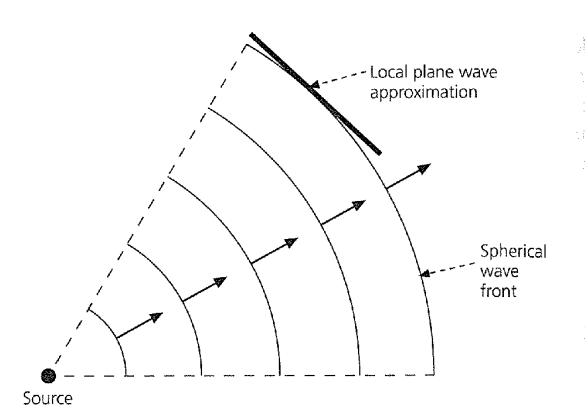
\includegraphics[width=0.4\textwidth]{assets/plane.png}
    \caption{At a far distance from the fault, the seismic waves can be validly approximated to plane waves.\cite{stein2009introduction}}
    \label{fig:plane}
\end{figure}

\begin{figure}
    \centering
    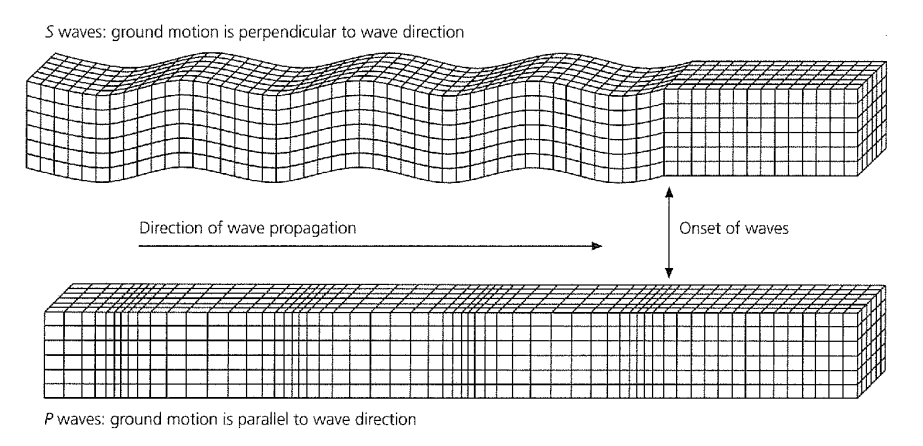
\includegraphics[width=\textwidth]{assets/s-p-waves.png}
    \caption{From \cite[Fig 2.4-3]{stein2009introduction}, a visual of the difference between $s$-waves and $p$-waves.}
    \label{fig:spwaves}
\end{figure}

\begin{figure}[ht]
    \centering
    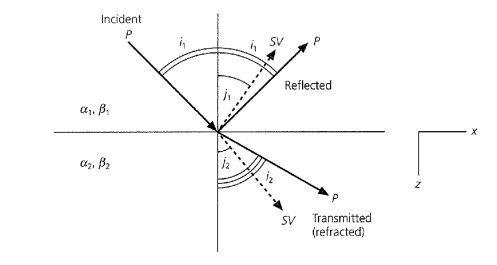
\includegraphics[width=.9\textwidth]
    {assets/pwave-reflected.PNG}
    \caption{A $p$-wave incident with angle $i_1$ to a boundary layer. The wave is partially reflected at angle $i_1$ and transmitted at angle $i_2$.\cite[Figure 2.5-5]{stein2009introduction}}
    \label{fig:reflection}
\end{figure}